\section{Auswertung}
\label{sec:Auswertung}

%Messwerte: Alle gemessenen physikalischen Größen sind übersichtlich darzustellen.


%Auswertung:
%Berechnung der geforderten Endergebnisse
%mit allen Zwischenrechnungen und Fehlerformeln, sodass die Rechnung nachvollziehbar ist.
%Eine kurze Erläuterung der Rechnungen (z.B. verwendete Programme)
%Graphische Darstellung der Ergebnisse.

Im Folgendem werden die während des Praktikums gemessenen Werte aufgeliset.
Die Messung der Resonanzfrequanz ergibt dann
    $35.6 \pm 0.2 \: \si{\kilo\hertz}$.

Messergebnisse für Aufgabe 1:
Für die Messungen von Aufgabe 1 werden hier jeweils die eingestellten Werte für die Kopplungskapazität $C_k$ aufgetragen, sowie die Frequenz bei der die Maxima gezählt wurden. Die gezählten Maxima und Extrema allgemein werden dahinter notiert. 

\begin{table}
  \centering
  \caption{Messwerte: Kopplungskapazität $C_k $ und Frequenz $f$ mit der entsprechenden Anzahl Maxima, sowie Extrema}
  \label{tab:schwebung}
  \begin{tabular}{c c c c}
    \toprule 
    $C_k \:/\: \si{\nano\farad}$ & $f \:/\: \si{\kilo\hertz}$ & Anzahl Maxima &  Anzahl Extrema   \\ 
    \midrule 
    0.997 & 0.626 & 2 & 3 \\
    2.290 & 0.626 & 3 & 5 \\
    2.860 & 0.626 & 5 & 9 \\
    4.740 & 0.626 & 6 & 12 \\
    6.860 & 0.626 & 9 & 17 \\
    8.180 & 0.626 & 11 & 23 \\
    9.990 & 0.626 & 13 & 25 \\
    12.000 & 0.626 & 18 & 35 \\
    \bottomrule
  \end{tabular}
\end{table}

\begin{figure}
  \centering
  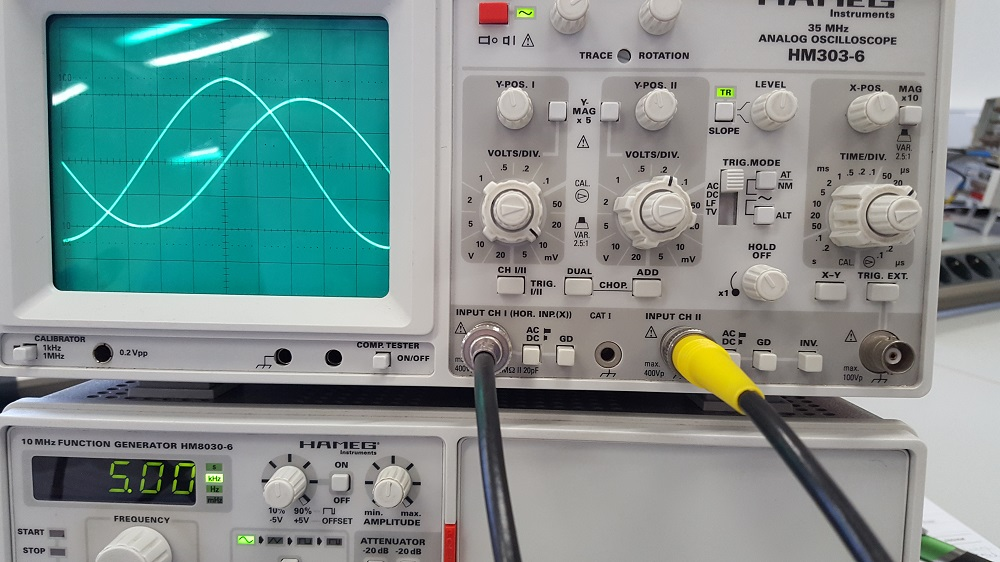
\includegraphics[width=\textwidth]{images/foto_03.jpg}
  \caption{Screenshot der Schwebung für den $C_k$ Wert $6.860$ aus \autoref{tab:schwebung}}
\end{figure}

Messergebnisse für Aufgabe 2:
In Aufgabe 2 wurden die Frequenzen für die jeweiligen Fundamentalschwingungen untersucht und gemessen, diese sind nachfolgend mit ihrer entsprechenden Kopplungskapazität $C_k$ aufgeschrieben.

\begin{table}
  \centering
  \caption{Messwerte: Kopplungskapazität $C_k $ und die Frequenzen $\nu _+$ und $\nu _-$}
  \label{tab:frequenzen}
  \begin{tabular}{c c c}
    \toprule 
    $C_k \:/\: \si{\nano\farad}$ & $\nu _+ \:/\: \si{\kilo\hertz}$ & $\nu _- \:/\: \si{\kilo\hertz}$   \\ 
    \midrule 
    0.997 & 35.7 & 56.1 \\
    2.190 & 35.7 & 46.5 \\
    2.86 & 35.7 & 44.3 \\
    4.740 & 35.7 & 41.2 \\
    6.860 & 35.7 & 39.6 \\
    8.180 & 35.7 & 39.1 \\
    9.990 & 35.7 & 38.5 \\
    12.000 & 35.7 & 38.1 \\
    \bottomrule
  \end{tabular}
\end{table}

Messergebnisse für Aufgabe 3:
In Abhängigkeit von der Kopplungskapazität $C_k$ sind die jeweilien maximalen Spannungsamplituden gelistet. Für jeden $C_k$ Wert wurde mit den beiden gemessenen Frequenzen aus \autoref{tab:frequenzen} die maximale Spannungsamplitude gemessen. Dabei entsprechen $U_{2+}$ und $U_{2-}$ der maximalen Spannungsamplitude im äußeren Schwingkreis bei den beiden Frequenzen $\nu _+$ und $\nu _-$. $U_k$ ist definiert als die maximale Spannungsamplitude innerhalb des gekoppelten Schwingkreises. Dort kann nur mit $\nu _-$ gemessen werden, da bei $\nu _+$, $C_k$ keinen Einfluss hat.

\begin{table}
  \centering
  \caption{Messwerte: Kopplungskapazität $C_k $ und Ampliduten von $U_{2+}$, $U_{2-}$ und $U_k$}
  \label{tab:amplituden}
  \begin{tabular}{c c c c}
    \toprule 
    $C_k \:/\: \si{\nano\farad}$ & $U_{2+} \:/\: \si{\volt}$ & $U_{2-} \:/\: \si{\volt}$ &  $U_k \:/\: \si{\volt}$       \\ 
    \midrule 
    2.190 & 2.50 & 2.00 & 2.50 \\
    2.860 & 2.50 & 2.25 & 2.75 \\
    4.740 & 2.50 & 2.25 & 2.75 \\
    6.860 & 2.50 & 2.25 & 2.75 \\
    8.180 & 2.50 & 2.38 & 2.75 \\
    9.990 & 2.50 & 2.38 & 2.88 \\
    12.000 & 2.50 & 2.50 & 2.88 \\
    \bottomrule
  \end{tabular}
\end{table}


Die Resonanzfrequanz kann nun mit der Formel für $\nu _+$ aus \autoref{eq:frequenzen} genau bestimmt werden.

Wobei:

$L = \SI{23.9540}{\milli\henry}$ 

und 

$C = \SI{0.7932}{\nano\farad}$

Hierbei wurde beachtet, dass die Induktivität $L$ ebenfalls eine Kapazität $C_{sp}$ besitzt, die in unserem Fall

$C_{sp} = \SI{0.0280}{\nano\farad}$ 

beträgt.
Bevor die Resonanzfrequenz $\nu _+$ berechnet werden kann, muss man also

$\SI{0.7932}{\nano\farad} + \SI{0.0280}{\nano\farad} = \SI{0.8212}{\nano\farad}$

als das neue $C$ setzen.
Damit ergibt sich dann der Theoriewert, der in der folgenden Tabelle mit dem gemessenen Wert verglichen wird.

\begin{table}
  \centering
  \caption{Vergleich der gemessenen Resonanzfrequanz und dem berechneten Theoriewert}
  \label{tab:resonanz}
  \begin{tabular}{c c}
    \toprule 
    Gemessener Wert $\nu _+ \:/\: \si{\kilo\hertz}$ & Berechneter Wert $\nu _+ \:/\: \si{\kilo\hertz}$    \\ 
    \midrule 
    35.600 & 35.884 \\
    \bottomrule
  \end{tabular}
\end{table}

Die Theoriewerte der berechneten Maxima aus Ausgabe 1 können mit der Formel \autoref{eq:extrema} berechnet werden. Die Werte für $\nu _+$ und $\nu _-$ sind die theoretisch berechneten Werte aus \autoref{tab:schwinungen}, für die jeweiligen Kopplungskapazitäten $C_k$, die man in der Aufgabe einstellt. Für die Anzahl der Maxima wurde jeweils auf den nächsten Runden Wert gerundet.

\begin{table}
  \centering
  \caption{Messwerte: Kopplungskapazität $C_k $ mit der gemessenen Anzahl Maxima und der theoretischen Anzahl Maxima }
  \label{tab:schwebungstheorie}
  \begin{tabular}{c c c}
    \toprule 
    $C_k \:/\: \si{\nano\farad}$ & gemessene Anzahl Maxima &  theoretische Anzahl Maxima   \\ 
    \midrule 
    0.997 & 2 & 2 \\
    2.290 & 3 & 3 \\
    2.860 & 5 & 4 \\
    4.740 & 6 & 7 \\
    6.860 & 9 & 9 \\
    8.180 & 11 & 11 \\
    9.990 & 13 & 13 \\
    12.000 & 18 & 16 \\
    \bottomrule
  \end{tabular}
\end{table}








Die in Aufgabe 2 gemessenen Frequenzen zu den Fundamentalschwingungen werden ebenfalls mit den Theoriewerten verglichen. Mithilfe der Formel für $\nu _-$ aus \autoref{eq:frequenzen} und den bekannten Werten für $L$ und $C$ kann besagte Frequenz bestimmt werden. Für $\nu_-$ ist jedoch die Kopplungskapazität $C_k$ nicht mehr irrelevant, sodass sich für jedes $C_k$ ein anderer Theoriewert ergibt.

\begin{table}
  \centering
  \caption{Vergleich der gemessenen Fundamentalschwingungen mit den berechneten Theoriewerten}
  \label{tab:schwingung}
  \begin{tabular}{c c c}
    \toprule 
    $C_k \:/\: \si{\nano\farad}$ & Gemessener Wert $\nu _- \:/\: \si{\kilo\hertz}$ & Berechneter Wert $\nu _- \:/\: \si{\kilo\hertz}$    \\ 
    \midrule 
    0.997 & 56.100 & 58.386 \\
    2.190 & 46.500 & 47.470 \\
    2.860 & 44.300 & 45.024 \\
    4.740 & 41.200 & 41.640 \\
    6.860 & 39.600 & 39.950 \\
    8.180 & 39.100 & 39.322 \\
    9.990 & 38.500 & 38.722 \\
    12.00 & 38.100 & 38.261 \\
    \bottomrule
  \end{tabular}
\end{table}





